\chapter{Durchführung der praktischen Untersuchungen}
\textbf{Kushagr Sinha}


Der experimentelle Teil lässt sich in zwei Versuche gliedern:

\begin{enumerate}
	\item \textbf{Lokalisation von Caspr2 an Synapsen:} Das Ziel war es,
	die Caspr2-Proteine sowohl an erregenden als auch an
	hemmenden Synapsen zu lokalisieren.
	\item \textbf{Einfluss von Caspr2-Antikörpern auf die
		Protein-Interaktion:} Spezifisch wurde untersucht, ob die
	Interaktion zum Protein Contactin-2 durch Caspr2-AK, gerichtet
	gegen die Discoidin- sowie Laminin1-Domänen, gestört wird.
\end{enumerate}

Um die Experimente beginnen zu können, wurden zunächst
Gehirnzellenkulturen, spezifisch Hippocampus-Neuronkulturen, benötigt. Dafür
werden aus einer trächtigen Maus die Embryonen entnommen, dekapitiert
und die Zellen aus der Hippocampus-Region des Gehirns entnommen.

%Die Zelldichte ist so hoch, dass sie zu Ungenauigkeiten führen würde. Daher wurden die Zellen voneinander getrennt und verdünnt. Dafür werden sie erst enzymatisch mit Trypsin behandelt, welches das Gewebe
%lockert, damit diese beim Triturieren nicht zerquetscht werden.
%Triturieren bezeichnet in diesem Zusammenhang das mechanische Vereinzeln
%von Zellen durch Auf- und Abpipettieren der Gewebestücke.

Um die Zellen aus dem dichten Gewebe voneinander zu trennen und zu vereinzeln, werden sie zuerst mit dem Enzym Trypsin behandelt. Trypsin spaltet die Peptidverbindungen zwischen den Zellen und lockert somit das Gewebe auf. Nach ca. fünf Minuten wird das Gewebe mit einem Medium (HBSS) gewaschen, das heißt, Lösung hinzugeben, kurz warten und schließlich abpipettieren, um das Enzym zu entfernen und die Enzymreaktion zu stoppen. Dadurch werden die Zellen beim anschließenden Triturieren (dem mechanischen Vereinzeln durch Auf- und Abpipettieren der Gewebestücke) nicht beschädigt.
%Danach werden diese mit einer Zellsuspensionslösung versetzt und auf die
%gewünschte Zelldichte verdünnt (ca.\ 20.000~Zellen/cm$^2$). Jetzt
%werden die Zellen auf Deckgläschen verteilt, welche vorher mit
%Poly-D-Lysin beschichtet wurden, um eine haftende Oberfläche für die
%Zellen zu schaffen. Damit die Zellen dann auch ein neuronales Netzwerk
%ausbilden, werden diese mit einem Neurobasal-Medium (NB), welches
%Nährstoffe und Wachstumsfaktoren enthält, versetzt und anschließend 14~Tage
%inkubiert.

Durch diesen Vorgang entsteht eine Zellsuspension, wobei die Zellen einzeln in dem Medium herumschweben (= Suspension). Mithilfe einer Zählkammer und verschiedener Berechnungen wird diese mit einem Medium verdünnt, um somit die gewünschte Zelldichte zu erreichen (ca.\ 20.000 Zellen/cm$^2$). Im Anschluss werden die Zellen auf Deckgläschen verteilt, welche vorher mit Poly-D-Lysin beschichtet wurden, um eine haftende Oberfläche für die Zellen zu schaffen. Damit die Zellen dann auch ein neuronales Netzwerk ausbilden, werden diese mit einem Neurobasal-Medium (NB), welches Nährstoffe und Wachstumsfaktoren enthält, versetzt und anschließend 14 Tage im Brutschrank bei 37 °C inkubiert. 

%Danach wurden die Zellen kurz vor dem Anfang der Färbungen 20 Minuten lang mit einer 4\%igen PFA-Lösung behandelt und damit fixiert. Fixieren bedeutet, die Proteine chemisch zu stabilisieren und die Zelle in ihrem aktuellen Zustand \glqq einzufrieren\grqq{}; allerdings stirbt die Zelle dabei.
% ────────────────────────────────────────────────────────────
\section{Untersuchung zur Lokalisation von Caspr2 an Synapsen}
% ────────────────────────────────────────────────────────────

%Der gesamte Prozess zur Immunfärbung der Zellkulturen dauerte drei Tage.
%Insgesamt wurden elf Deckgläschen verwendet (siehe Tabelle~\ref{tab:proben}), welche
%in verschiedene Versuchsgruppen unterteilt wurden. Am ersten Tag
%wurden die Zellen nach dem Fixieren dreimal gewaschen, das heißt Lösung hinzugeben, kurz warten und dann abpipettieren (siehe Abbildung \ref{fig:waschV}). Dies wurde immer mit PBS (Phosphat-gepufferte Salzlösung) gemacht. Das PBS wurde benutzt, da es eine isotonische, nicht-toxische Lösung ist,
%die den pH-Wert stabilisiert und die Zellen schont.


Der gesamte Prozess zur Immunfärbung der Zellkulturen dauerte drei Tage.
Insgesamt wurden elf Deckgläschen verwendet (siehe Tabelle~\ref{tab:proben}), welche
in verschiedene Versuchsgruppen unterteilt wurden. 

Am ersten Tag wurden die Zellen kurz vor dem Anfang der Färbungen 20 Minuten lang mit einer 4\%igen PFA-Lösung behandelt und damit fixiert. Fixieren bedeutet, die Proteine chemisch zu stabilisieren und die Zelle in ihrem aktuellen Zustand \glqq einzufrieren\grqq{}; allerdings stirbt die Zelle dabei. Darauffolgend wurden sie dreimal mit PBS (Phosphat-gepufferte Salzlösung) gewaschen (siehe Abbildung \ref{fig:waschV}). Das PBS wurde benutzt, da es eine isotonische, nicht-toxische Lösung ist, die den pH-Wert stabilisiert und die Zellen schont.

Nachdem die Zellen dreimal gewaschen wurden, wurde ein Puffer~B1
aufgetragen, welcher aus 10\%iger BSA-Lösung (Rinderserumalbumin) und
10\%iger NDS-Lösung (normales Eselserum) bestand und als
Blockierungslösung diente. Dabei dient der Puffer dazu, unspezifische
Bindungsstellen auf den Deckgläschen und auf den Zellen zu besetzen. Dies
stellt sicher, dass die später hinzugefügten AK nur an ihre spezifischen
Zielproteine binden und keine störende Hintergrund-Fluoreszenz verursachen.

Nach einer Stunde Einwirkzeit wurde der Puffer~B1 abpipettiert und die
ersten Primärantikörper (Caspr2 bzw.\ der Kontrollantikörper)
hinzugefügt. Diese wurden anschließend über Nacht bei 4\,°C
inkubiert.

% ── Bild 1 ausgelassen ───────────────────────────────────────
\clearpage
\begin{table}[htbp]
	\centering
	\caption{Übersicht der elf Proben des ersten Versuches.}
	\label{tab:proben}
	\setlength{\tabcolsep}{3pt} % Verringert den seitlichen Abstand in den Zellen
	\begin{tabularx}{\textwidth}{c >{\raggedright\arraybackslash}X c >{\raggedright\arraybackslash}X c >{\raggedright\arraybackslash}X}
		\toprule
		\textbf{Nr.} & \textbf{Färbung} &
		\textbf{Nr.} & \textbf{Färbung} &
		\textbf{Nr.} & \textbf{Färbung} \\
		\midrule
		(1) & Caspr2 + VGlut1 &
		(5) & Caspr2 + VGat &
		(9) & Kontrolle + VGlut1 \\
		(2) & Caspr2 + VGlut1 &
		(6) & Caspr2 + VGat &
		(10) & Kontrolle + VGat \\
		(3) & Caspr2 + VGlut1 &
		(7) & Caspr2 + VGat &
		(11) & Negativkontrolle (nur SEK1+2) \\
		(4) & Caspr2 + VGlut1 &
		(8) & Caspr2 + VGat &
		& \\
		\bottomrule
	\end{tabularx}
\end{table}

\begin{figure}[h]
	\centering
	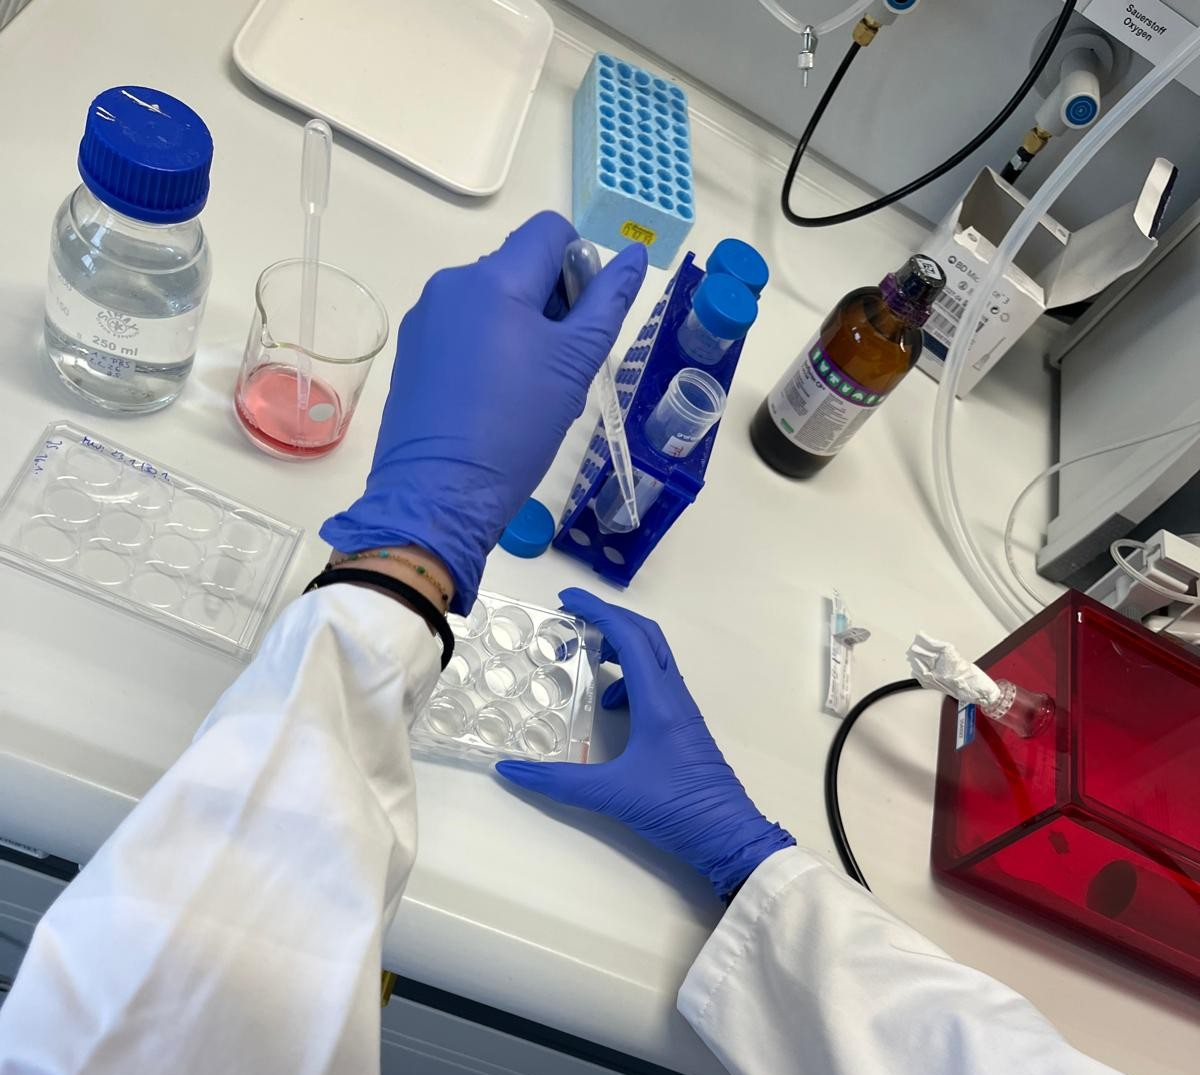
\includegraphics[width=0.75\textwidth]{abbildungen/waschvorgangDPU.jpeg}
	\caption{Vorgang des Fixierens und Waschens \parencite{eigenAu6.1}}
	\label{fig:waschV}
\end{figure}
Am zweiten Tag wurden die Deckgläschen in eine Feuchtekammer
transferiert. Dies ist notwendig, damit die geringen Mengen an
Antikörperlösung während der Einwirkzeit nicht verdunsten und die Zellen nicht austrocknen. Die Kammer
bestand aus einer Plastikbox mit angefeuchteten Papiertüchern als
Untergrund (siehe Abbildung \ref{fig:fKammer}).
\clearpage
% (siehe Bild 2)
\begin{figure}[h]
	\centering
	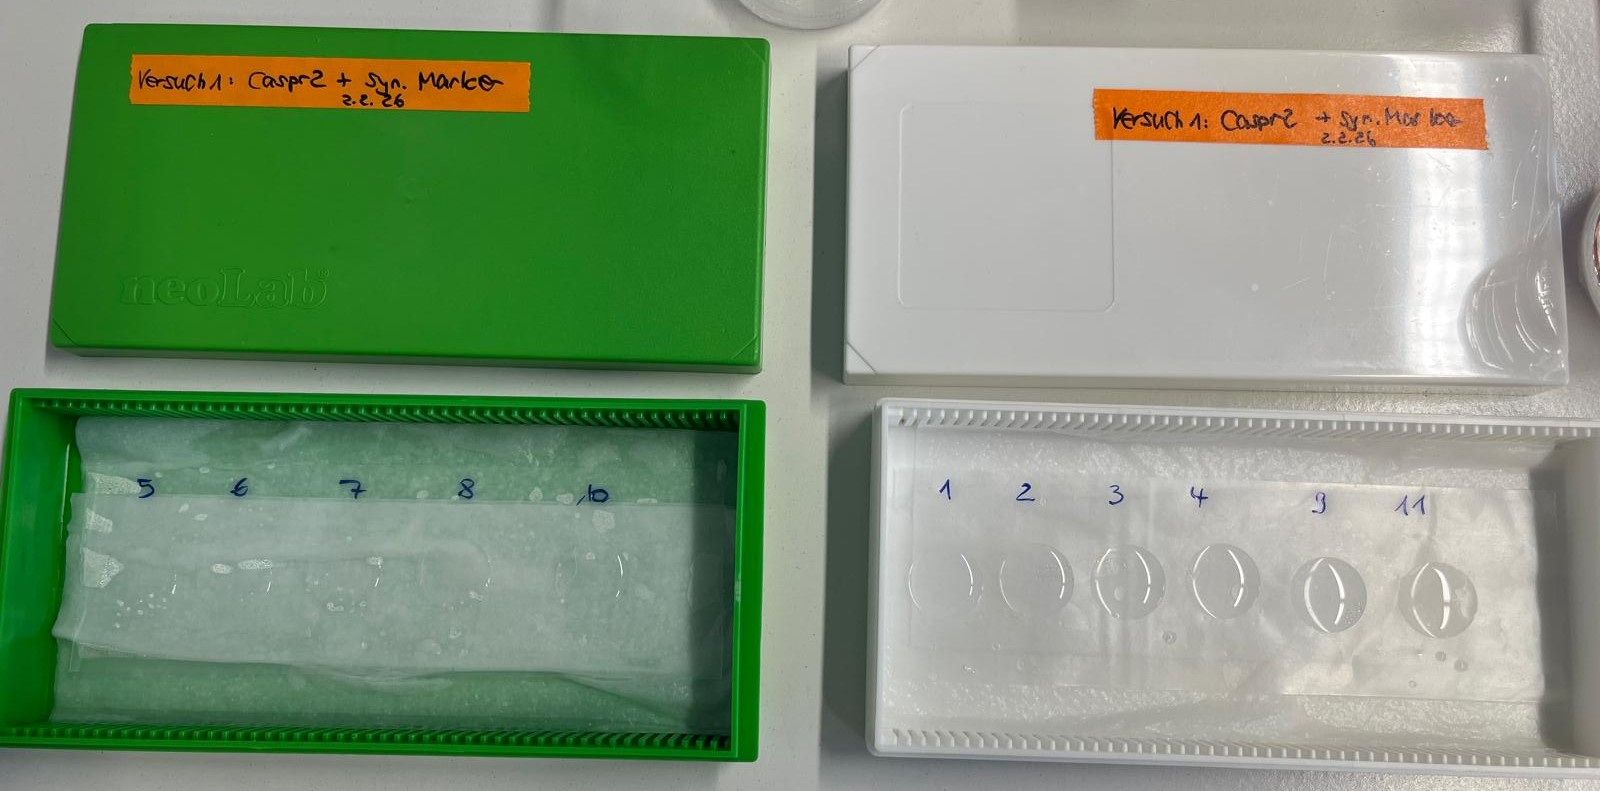
\includegraphics[width=1\textwidth]{abbildungen/fkammerDPU.jpeg}
	\caption{Feuchtekammer \parencite{eigenAu6.2}}
	\label{fig:fKammer}
\end{figure}

Nach sechsmaligem Waschen mit PBS wurden die ersten Sekundärantikörper, nämlich AF647@sheep, hinzugegeben. Die Bezeichnung \glqq AF647\grqq{} gibt dabei an, dass der Antikörper mit dem Fluoreszenzfarbstoff AF647 markiert ist, der bei einer Wellenlänge von 647 nm emittiert. \glqq Sheep\grqq{} bezeichnet hingegen die Spezies, gegen die die Sekundärantikörper gerichtet sind. Da der erste Primärantikörper gegen Caspr2 gerichtet ist und aus dem Schaf stammt, bindet der gegen Schaf gerichtete Sekundärantikörper an diesen Primärantikörper. Nach einer Inkubationszeit von zwei Stunden wurde die Deckgläschen erneut sechsmal mit PBS gewaschen.

%Um die Zellen für die zweiten Primärantikörper besser zugänglich zu
%machen, wurde eine Pufferlösung~B2 hergestellt. Diese bestand aus der
%B1-Lösung und zusätzlich Triton. Das Triton dient dazu, kleine Löcher
%in die Zellmembran zu machen, damit die VGlut/VGat-Antikörper auch in
%das Innere der Synapse gelangen und binden können. Diese wurden nach der
%Puffer-Behandlung hinzugefügt und erneut über Nacht bei 4\,°C gelagert.

Wichtige Proteine von Synapsen sind VGlut und VGat. Da sich diese allerdings nicht auf der Membranoberfläche, sondern im Inneren der Zelle befinden, muss erst ein Zugang durch die fixierte Zellmembran geschaffen werden, damit die Antikörper daran binden können.

Um die Zellen für diese Antikörper zugänglich zu machen, wurde die Pufferlösung B2 hergestellt. Diese bestand aus der B1-Lösung und zusätzlich dem Detergenz Triton. Triton wirkt ähnlich wie Seife und kann Fette lösen. Da die Zellmembran aus Fettsäuren besteht, \glqq wäscht\grqq{} das Triton kleine Löcher in die Membran. So können die VGlut- und VGat-Antikörper, die in Meerschweinchen gezüchtet wurden, in das Innere der Synapse gelangen und binden. Die Zugabe erfolgte nach der Puffer-Behandlung mit anschließender Inkubation über Nacht bei 4\,°C.

Am dritten Tag wurde die Lösung wieder sechsmal mit PBS abgewaschen, und
es folgte die Zugabe der zweiten Sekundärantikörper, CF488@gp (fluoresziert
grün und ist gerichtet gegen Meerschweinchen-AK), gegen VGlut- und
VGat-AK. Nach zwei Stunden wurde sechsmal abgewaschen.

Anschließend wurde DAPI hinzugefügt, eine Lösung, die den Zellkern
anfärbt, indem sie mit der darin vorhandenen DNA interagiert. Damit wurde erzielt, dass die Zellen unter dem Mikroskop einfacher zu finden sind.

Diese wurden dann dreimal gewaschen. Zehn Minuten lang wurden die
Präparate dann nochmals mit einer 4\%igen PFA-Lösung fixiert, damit sie über Monate hinweg
mikroskopiert werden können. Nach einem letzten Waschschritt waren die
Präparate fertig für die Auswertung.

\section{Untersuchung zum Einfluss von humanen Caspr2-Antikörpern auf die Protein-Interaktion mit Contactin-2}

Im zweiten Versuchsteil wurde untersucht, ob die Bindung von humanen Caspr2-Antikörpern (aus Patientenseren) die Interaktion zwischen Caspr2 und dem Bindungspartner Contactin-2 beeinträchtigt oder blockiert.
Der Ablauf gliederte sich erneut in drei Tage mit mehreren Aufbereitungsschritten.

%

%Der erste Tag der Färbungen fing damit an dass die noch lebenden Zellen mit den zuvor erwähnten humanen AK behandelt wurden. DAbei gab es 2 verschieden ARten, eine die daen Laminin1 Domänene angegriffen ahben und die anderen die den Discoidin Domäne angegriffen haebn. Damit entstanden insgesamt 12 PRoben wie in Tabelle \ref{tab:proben2} zu sehen sind.

%Zu Beginn wurden die benötigten Neurobasal-Medien vorbereitet und auf 37 °C erwärmt. Für die Behandlung der Neuronenkulturen wurden drei verschiedene Ansätze hergestellt. Für die Discoidin gerichteten AK wurden 20 µl Discoidin mit 2600 µl Neurobasal-Medium versetzt. Für die Laminin-Bedingung wurden 17,93 µl Laminin mit 2600 µl Neurobasal-Medium gemischt. Als Kontrolle wurden 10,83 µl MGO-53 mit 1300 µl Neurobasal-Medium angesetzt. Anschließend wurden die entsprechenden Ansätze zu den Neuronenkulturen gegeben. Die Kulturen wurden für 24 Stunden bei 37 °C inkubiert.


Zu Beginn des ersten Tages des Versuches wurde zur Vorbereitung Neurobasal-Medium auf 37 \,°C erwärmt. Damit konnten die verschiedenen benötigten Ansätze mit humanen monoklonalen Caspr2-Antikörpern gegen Discoidin oder Laminin-1 hergestellt werden. Außerdem gab es noch einen Kontroll-Antikörper, mgo-53, mit demselben Ziel wie im ersten Versuch genannt.

 Als diese Primär-Antikörper mit dem Neurobasal-Medium auf die benötigte Konzentration verdünnt wurden, wurden jeweils 500 µl in jedes Well getropft. Anschließend wurden sie bei 37 \,°C 24 Stunden lang inkubiert. Damit entstanden insgesamt 12 Proben, wie in Tabelle \ref{tab:proben2} zu sehen ist.

\begin{table}[htbp]
	\centering
	\caption{Übersicht der zwölf Proben des zweiten Versuches.}
	\label{tab:proben2}
	\setlength{\tabcolsep}{3pt} % Verringert den seitlichen Abstand in den Zellen
	\begin{tabularx}{\textwidth}{c >{\raggedright\arraybackslash}X c >{\raggedright\arraybackslash}X c >{\raggedright\arraybackslash}X}
		\toprule
		\textbf{Nr.} & \textbf{Färbung} &
		\textbf{Nr.} & \textbf{Färbung} &
		\textbf{Nr.} & \textbf{Färbung} \\
		\midrule
		(1) & Discoidin + Contactin-2 &
		(5) & Laminin1 + Contactin-2 &
		(9) & Control + Contactin-2 \\
		(2) & Discoidin + Contactin-2 &
		(6) & Laminin1 + Contactin-2 &
		(10) & Control + Contactin-2 \\
		(3) & Discoidin + Contactin-2 &
		(7) & Laminin1 + Contactin-2 &
		(11) & negative control (nur SEK1+2) \\
		(4) & Discoidin + Contactin-2 &
		(8) & Laminin1 + Contactin-2 &
		(12) & negative control (nur SEK1+2) \\
		\bottomrule
	\end{tabularx}
\end{table}
Am zweiten Tag der Färbung wurden die Neuronen auf den Deckgläschen zunächst dreimal kurz bei 37\,°C mit erwärmtem Neurobasal-Medium gewaschen. Anschließend wurden die Zellen für 20~Minuten bei Raumtemperatur mit einer 4\,\%igen PFA-Lösung behandelt, um sie in ihrem aktuellen Zustand zu fixieren und chemisch zu stabilisieren. Nach der Fixierung folgte ein dreimaliger Waschschritt mit PBS für jeweils 5~Minuten, um Reste des Fixiermittels gründlich zu entfernen.

Zur Vermeidung unspezifischer Antikörperbindungen wurden die Präparate danach für eine Stunde bei Raumtemperatur mit dem Puffer B1 inkubiert. Dieser bestand aus einer Mischung aus 10\,\%iger BSA-Lösung und 10\,\%igem NGS (normales Ziegenserum / Normal Goat Serum) in PBS. Das NGS blockiert, genau wie das NDS im vorherigen Versuch, die freien Bindungsstellen auf der Oberfläche.




Da die Zellen bereits mit humanen Caspr2-Antikörpern behandelt worden waren, folgte im nächsten Schritt direkt die Zugabe des ersten Sekundärantikörpers. Hierfür wurde der Puffer SEK1, bestehend aus 1\,\% BSA, 1\,\% NGS und dem Antikörper CF640R@hu, aufgetragen und für 2~Stunden bei Raumtemperatur inkubiert. Der Antikörper CF640R@hu ist spezifisch gegen humane Antikörper gerichtet und trägt den Fluoreszenzfarbstoff CF640R (Emissionswellenlänge im fernroten Bereich bei ca.~640\,nm), wodurch die gebundenen Caspr2-Antikörper sichtbar gemacht werden.

Nach Ablauf der Inkubationszeit wurden die Deckgläschen sechsmal für jeweils 5~Minuten mit PBS gewaschen. Danach wurde der Puffer PRIM2 aufgetragen, welcher den gegen Contactin-2 gerichteten Primärantikörper (in Kaninchen gezüchtet) sowie 1\,\% BSA und 1\,\% NGS enthielt. Die Inkubation erfolgte über Nacht bei 4\,°C in der Feuchtekammer.

Am darauffolgenden Tag wurden die Proben erneut sechsmal für jeweils 5~Minuten mit PBS gewaschen, um ungebundene Contactin-2-Antikörper zu entfernen. Im Anschluss wurde der zweite Sekundärantikörper über den Puffer SEK2 (1\,\% BSA, 1\,\% NGS und CF568@rb) hinzugegeben. Dieser Antikörper bindet spezifisch an Kaninchen-Antikörper und fluoresziert durch den Farbstoff CF568 in roter Farbe. Die Inkubationszeit betrug zwei Stunden bei Raumtemperatur.

Nach erneutem sechsmaligem Waschen mit PBS wurde für 5~Minuten DAPI hinzugefügt. DAPI diente wieder als Orientierungshilfe bei der Mikroskopie. Nach drei kurzen Waschschritten mit PBS wurden die Präparate nochmals für 10~Minuten bei Raumtemperatur mit einer 4\,\%igen PFA-Lösung nachfixiert, um die gebildeten Antikörper-Protein-Komplexe dauerhaft zu stabilisieren.
\clearpage
Nach drei finalen kurzen Waschschritten mit PBS wurden die Deckgläschen, aus dem ersten Versuch sowie dem zweiten Versuch, schließlich mit dem Eindeckmedium Fluoromount auf Objektträgern eingedeckt (siehe Abbildung \ref{fig:objtr}). Fluoromount schützt das Präparat vor dem Austrocknen und verhindert das Ausbleichen der Fluoreszenzfarbstoffe, sodass die Proben mithilfe des SIM-Mikroskops ausgewertet werden können.
\begin{figure}[h]
	\centering
	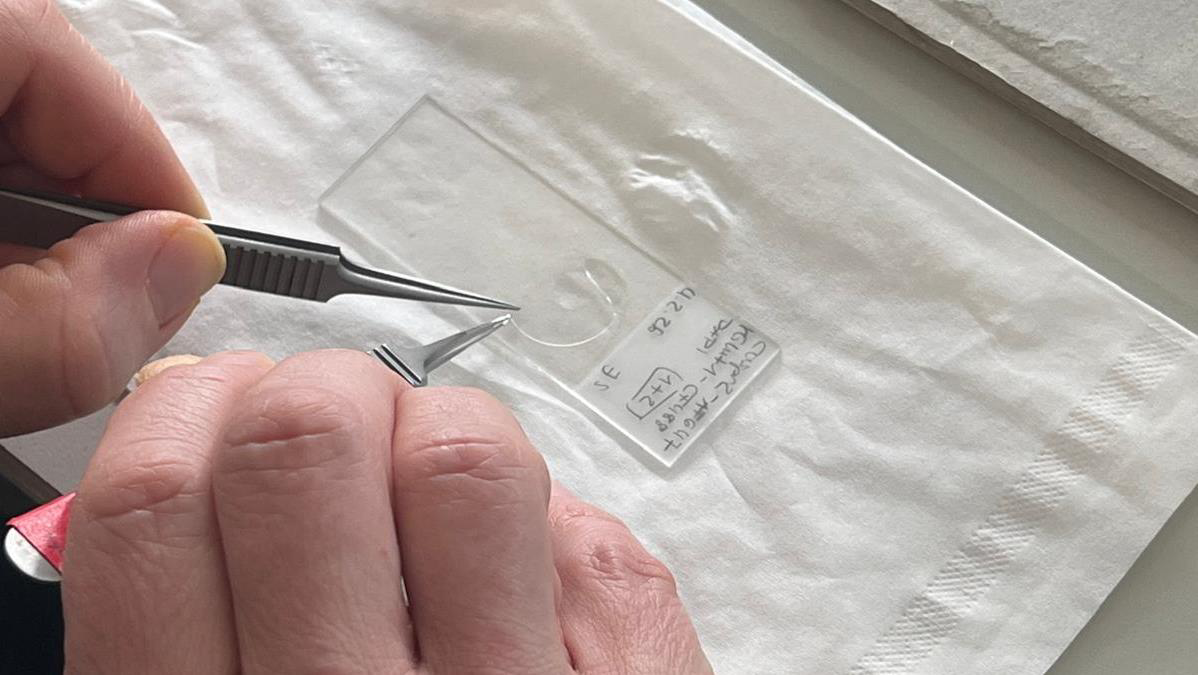
\includegraphics[width=1\textwidth]{abbildungen/objektträgerDPU.png}
	\caption{Feuchtekammer \parencite{eigenAu6.3}}
	\label{fig:objtr}
\end{figure}

